\paragraph{Sơ đồ tuần tự luồng quản lý nhân vật}

Luồng nghiệp vụ này mô tả
quy trình quản trị viên
(Admin)
thực hiện tạo mới hoặc cập nhật một nhân vật,
bao gồm các bước tải lên tài nguyên ảnh đại diện,
âm thanh giới thiệu lên Supabase Storage
và cập nhật thông tin cấu hình vào Persona Database.

\begin{figure}[H]
\centering
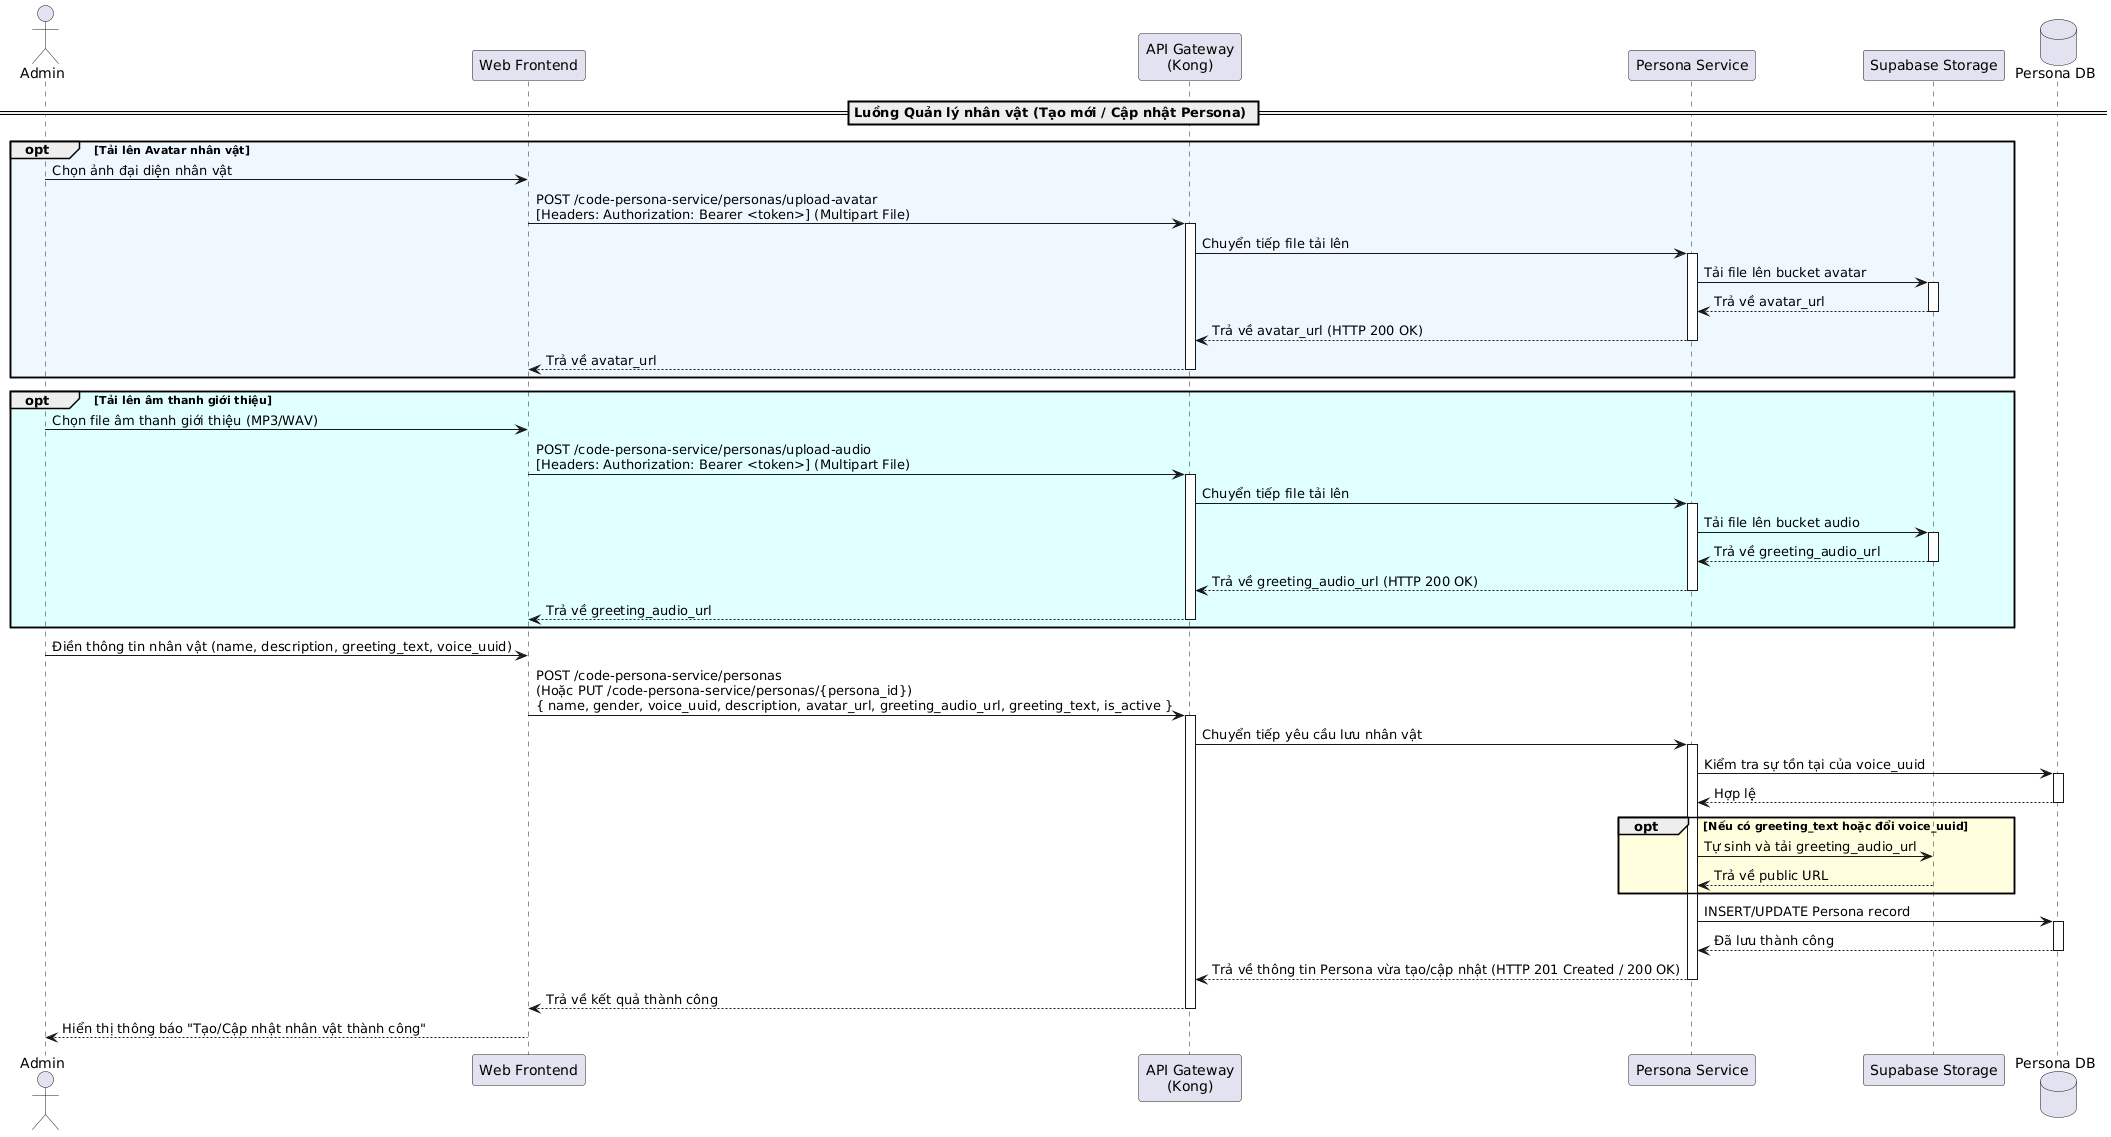
\includegraphics[width=0.95\textwidth]{contents/Sequence/UML-Sequence-AdminManagePersona.png}
\caption{Sơ đồ tuần tự luồng quản lý nhân vật}
\end{figure}

\begin{table}[H]
\centering
\renewcommand{\arraystretch}{1.3}

\begin{tabular}{|l|l|p{5cm}|}
\hline
\textbf{Thành phần} & \textbf{Phân loại} & \textbf{Vai trò trong hệ thống} \\ \hline
Admin & Actor & Quản trị viên
hệ thống có quyền tạo, sửa và cấu hình nhân vật. \\ \hline
Web Frontend & Component & Giao diện web Next.js. \\ \hline
API Gateway (Kong) & Component & Cổng API chuyển tiếp các yêu cầu API. \\ \hline
Persona Service & Microservice & Tiếp nhận yêu cầu, xử lý nghiệp vụ, kiểm tra tính hợp lệ của giọng nói liên kết và lưu trữ. \\ \hline
Supabase Storage & External Service & Nền tảng lưu trữ file avatar và audio giới thiệu của nhân vật. \\ \hline
Persona Database & Database & CSDL lưu trữ thông tin cấu hình nhân vật và liên kết giọng nói. \\ \hline
\end{tabular}
\caption{Các thành phần tham gia luồng quản lý nhân vật}
\end{table}

\subparagraph{Mô tả tổng quan}

\begin{itemize}

\item \textbf{Tải lên ảnh đại diện (Tùy chọn):}
Quản trị viên
tải lên ảnh đại diện mới cho nhân vật.
Giao diện gửi tệp tin qua cổng API tới dịch vụ nhân vật.
Dịch vụ lưu trữ ảnh và trả lại liên kết ảnh đại diện.

\item \textbf{Tải lên âm thanh giới thiệu (Tùy chọn):}
Quản trị viên
tải lên tệp âm thanh giới thiệu.
Giao diện gửi yêu cầu tải âm thanh, dịch vụ nhân vật lưu tệp và phản hồi liên kết âm thanh giới thiệu.

\item \textbf{Lưu thông tin nhân vật:}
Quản trị viên
điền các cấu hình của nhân vật và
gửi yêu cầu lưu hoặc cập nhật thông tin qua giao diện.

\item \textbf{Xử lý và lưu trữ:}
Dịch vụ nhân vật kiểm tra tính hợp lệ của giọng nói được chọn.
Nếu có nội dung văn bản giới thiệu hoặc thay đổi giọng nói, hệ thống tự động tạo lại tệp âm thanh giới thiệu tương ứng,
cập nhật liên kết âm thanh và lưu toàn bộ thông tin nhân vật vào CSDL.
\end{itemize}
